\documentclass[conference]{IEEEtran}

\usepackage[T1]{fontenc}
\usepackage[utf8]{inputenc}
\usepackage{amsmath,amssymb}
\usepackage{graphicx}
\usepackage{subcaption}
\usepackage{booktabs}
\usepackage{siunitx}
\usepackage{url}
\usepackage[hidelinks]{hyperref}

\sisetup{separate-uncertainty=true,detect-all=true}
\graphicspath{{img/}}

\begin{document}

\title{Assembly and Characterization of a Galileoscope:\\
Magnification, Field of View and Exit Pupil}

\author{\IEEEauthorblockN{Nicol\'as Seguel}
\IEEEauthorblockA{Laboratorio de Instrumentación Astronómica -- IEE3873\\
Pontificia Universidad Cat\'olica de Chile\\
\texttt{neseguel@uc.cl}}}

\maketitle

\section{Introduction}

The instrument characterized in this experiment is a Galileoscope, a kit
refractor with a \SI{50}{\milli\meter} achromatic objective of
\SI{500}{\milli\meter} focal length ($f/10$). The kit provides a
\SI{20}{\milli\meter} eyepiece, which gives a nominal magnification of
$25\times$, and a $2\times$ Barlow tube that extends the effective
focal length to give $50\times$~\cite{galileoscope}. The telescope was
assembled from the parts in the box following the supplied instructions, and
then measured as an optical system: magnification $M$, field of view (FOV) and
exit pupil diameter $D_{ex}$.

Two independent methods were used. The first is afocal photography: a
\SI{30}{\centi\meter} ruler was fixed to a tripod at a measured distance
$L = \SI{18.7}{\meter}$ from the telescope, and a phone camera photographed it
twice, once directly and once through the eyepiece with the camera lens placed
at the exit pupil. Because the camera settings are the same in both frames, the
ratio of the pixel lengths of the same physical object gives the angular
magnification directly,
\begin{equation}
M = \frac{\theta_i}{\theta_o} = \frac{d_{px,tel}}{d_{px,dir}} ,
\label{eq:M}
\end{equation}
without any pixel-to-metre calibration. The same pair of frames also gives the
field of view: the ruler spans the full illuminated field of the eyepiece, so
the angular width of the field is
\begin{equation}
\mathrm{FOV} = 2\arctan\!\left(\frac{W}{2L}\right),
\label{eq:fov}
\end{equation}
with $W = \SI{30}{\centi\meter}$.

The second method uses the exit pupil. In an afocal system the magnification is
the ratio of the entrance to the exit pupil diameters,
\begin{equation}
M = \frac{D_{obj}}{D_{ex}} .
\label{eq:pupil}
\end{equation}
The $25\times$ and $50\times$ configurations are Keplerian, so the
exit pupil is real and can be projected: illuminating the objective and moving
a sheet of paper behind the eyepiece produces a bright disc whose diameter is
minimum at the exit pupil plane. This method is geometric and does not depend
on the camera, so it acts as a cross-check of \eqref{eq:M}.

Section~\ref{sec:equip} lists the equipment, Section~\ref{sec:meas} reports the
measurements, Section~\ref{sec:disc} discusses the scatter and the systematic
effects, and Section~\ref{sec:concl} summarizes the results.

\section{Equipment, Materials and Instruments}
\label{sec:equip}

Table~\ref{tab:equip} lists everything used during the session. The telescope
and the target were mounted on separate tripods so that both could be aligned
and left fixed for the whole set of repetitions.

\begin{table}[htbp]
\caption{Equipment used in the experiment.}
\label{tab:equip}
\centering
\small
\begin{tabular}{@{}ll@{}}
\toprule
\textbf{Item} & \textbf{Use} \\
\midrule
Galileoscope (\SI{50}{\milli\meter} $f/10$) & instrument under test \\
Photographic tripod & telescope mount \\
Second tripod & target (ruler) mount \\
\SI{30}{\centi\meter} ruler (mm graduation) & target of known length \\
Measuring tape (\SI{30}{\meter}, mm) & telescope--target distance $L$ \\
Vernier caliper (\SI{0.05}{\milli\meter}) & $D_{obj}$ and $D_{ex}$ \\
Phone camera & afocal and direct imaging \\
Phone flashlight & illumination of the objective \\
Sheet of white paper & screen for the exit pupil \\
\bottomrule
\end{tabular}
\end{table}

\section{Measurements}
\label{sec:meas}

\subsection{Magnification by afocal photography}

The telescope was set at $L = \SI{18.7}{\meter}$ from the ruler and five
independent pairs of frames were taken with the $25\times$ eyepiece,
re-centring the camera on the eyepiece between pairs. Fig.~\ref{fig:photos}
shows one such pair. The length of the ruler was measured in pixels in both
frames; the results are in Table~\ref{tab:mag}, where the per-trial
uncertainty comes from propagating a $\pm 1$\,px reading error through
\eqref{eq:M}.

\begin{figure}[htbp]
\centering
\begin{subfigure}[b]{0.485\linewidth}
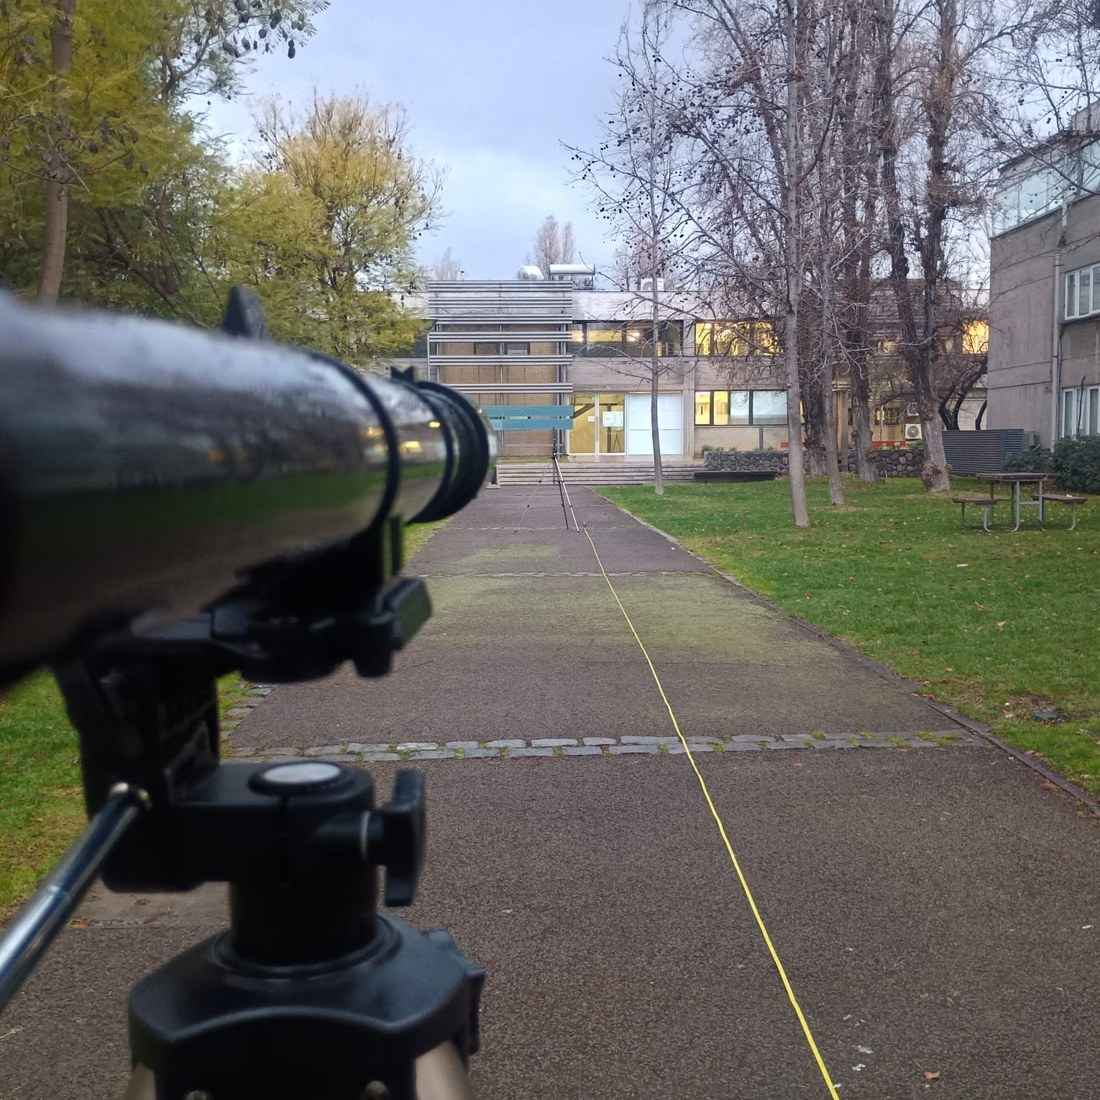
\includegraphics[width=\linewidth]{setup_direct.jpg}
\caption{}
\end{subfigure}
\hfill
\begin{subfigure}[b]{0.485\linewidth}
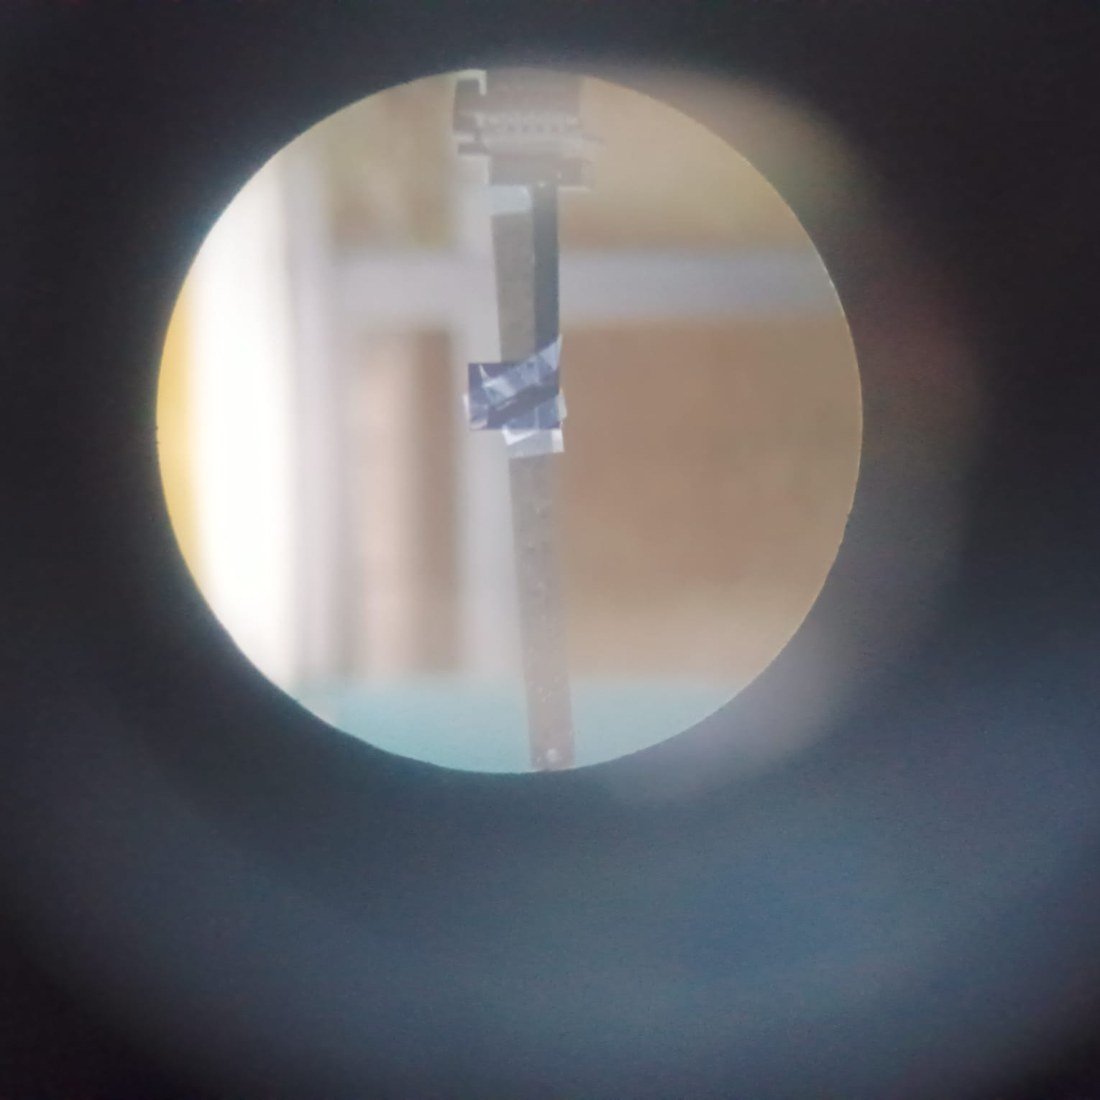
\includegraphics[width=\linewidth]{afocal_25x.jpg}
\caption{}
\end{subfigure}
\caption{(a) Direct frame: telescope on its tripod, the measuring tape along
the ground and the target tripod at \SI{18.7}{\meter}. (b) Afocal frame of the
same target through the $25\times$ eyepiece; the image is inverted and the
ruler fills the illuminated field.}
\label{fig:photos}
\end{figure}

\begin{table}[htbp]
\caption{Pixel length of the \SI{30}{\centi\meter} ruler in the direct and
afocal frames, and the resulting magnification.}
\label{tab:mag}
\centering
\small
\begin{tabular}{@{}ccccc@{}}
\toprule
\textbf{Trial} & $d_{px,dir}$ [px] & $d_{px,tel}$ [px] & $M_i$ & $\sigma_{M_i}$ \\
\midrule
1 & 33 & 815 & 24.70 & 0.75 \\
2 & 32 & 796 & 24.88 & 0.78 \\
3 & 34 & 779 & 22.91 & 0.68 \\
4 & 32 & 811 & 25.34 & 0.79 \\
5 & 33 & 803 & 24.33 & 0.74 \\
\midrule
\multicolumn{3}{@{}l}{Mean $\bar{M}$} & \multicolumn{2}{r@{}}{$24.43$} \\
\multicolumn{3}{@{}l}{Sample deviation $s$} & \multicolumn{2}{r@{}}{$0.92$} \\
\multicolumn{3}{@{}l}{Error of the mean $s/\sqrt{N}$} & \multicolumn{2}{r@{}}{$0.41$} \\
\bottomrule
\end{tabular}
\end{table}

The five values are plotted in Fig.~\ref{fig:mag}. The result is
\begin{equation}
M_{25\times} = 24.43 \pm 0.41 ,
\end{equation}
which sits $1.4\sigma$ below the nominal $25\times$.

\begin{figure}[htbp]
\centering
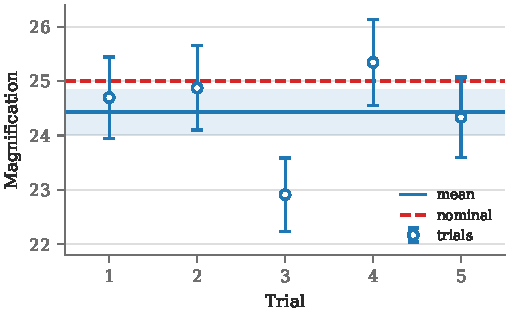
\includegraphics[width=\linewidth]{fig_magnification.pdf}
\caption{Per-trial magnification with the $\pm 1$\,px propagated error. The
solid line is the mean and the band its standard error; the dashed line is the
nominal value.}
\label{fig:mag}
\end{figure}

\subsection{Field of view}

In the afocal frames the \SI{30}{\centi\meter} ruler spans the illuminated
field of the eyepiece, so $W = 300 \pm 10$\,mm is taken as the field width at
$L = 18.7 \pm 0.3$\,m. From \eqref{eq:fov},
\begin{equation}
\mathrm{FOV}_{25\times} = 16.04 \pm 0.59\ \mathrm{mrad}
= 0.919^\circ \pm 0.034^\circ ,
\end{equation}
that is $3309'' \pm 122''$. Combined with the measured magnification, the
apparent field seen by the observer is
$\mathrm{AFOV} = M \cdot \mathrm{FOV} = 22.5^\circ \pm 0.9^\circ$, a value
consistent with a simple two-element eyepiece.

\subsection{Exit pupil projection}

The objective clear aperture was measured with the caliper, and the exit pupil
was projected on a sheet of paper using the phone flashlight as the source,
sliding the paper until the disc reached its minimum diameter. Five readings
were taken for each quantity; only the $25\times$ and $50\times$
configurations were measured this way. The data are in Table~\ref{tab:pupil}
and compared with the expected values in Fig.~\ref{fig:pupil}.

\begin{table}[htbp]
\caption{Caliper readings of the objective aperture and of the projected exit
pupil, in mm.}
\label{tab:pupil}
\centering
\small
\begin{tabular}{@{}lccccccc@{}}
\toprule
\textbf{Quantity} & 1 & 2 & 3 & 4 & 5 & Mean & $s/\sqrt{N}$ \\
\midrule
$D_{obj}$        & 47.1 & 47.0 & 47.2 & 47.3 & 47.1 & 47.14 & 0.05 \\
$D_{ex}$ ($25\times$) & 1.00 & 0.90 & 0.80 & 1.00 & 1.00 & 0.94 & 0.04 \\
$D_{ex}$ ($50\times$) & 0.50 & 0.40 & 0.60 & 0.66 & 0.52 & 0.54 & 0.04 \\
\bottomrule
\end{tabular}
\end{table}

\begin{figure}[htbp]
\centering
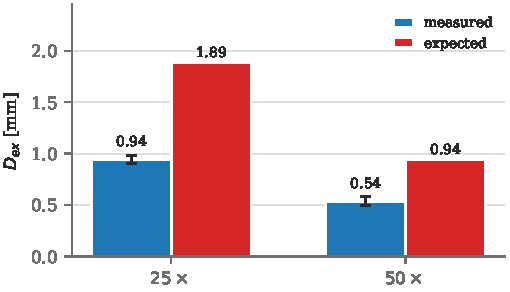
\includegraphics[width=\linewidth]{fig_pupil.pdf}
\caption{Measured exit pupil against the value expected from the nominal
magnification, $D_{obj}/M_{nom}$, for both Keplerian configurations.}
\label{fig:pupil}
\end{figure}

Applying \eqref{eq:pupil} with the relative errors added in quadrature,
\begin{align}
M_{25\times}^{proj} &= 50.2 \pm 2.1 , \\
M_{50\times}^{proj} &= 88.0 \pm 7.3 .
\end{align}

Table~\ref{tab:summary} collects the results of both methods.

\begin{table}[htbp]
\caption{Summary of the measured parameters.}
\label{tab:summary}
\centering
\small
\begin{tabular}{@{}lccc@{}}
\toprule
\textbf{Parameter} & $\mathbf{25\times}$ & $\mathbf{50\times}$ & \textbf{Nom.} \\
\midrule
$M$ (photographic) & $24.43 \pm 0.41$ & --- & 25 / 50 \\
$M$ (projection)   & $50.2 \pm 2.1$   & $88.0 \pm 7.3$ & 25 / 50 \\
FOV                & $0.919^\circ \pm 0.034^\circ$ & --- & --- \\
$D_{ex}$ [mm]      & $0.94 \pm 0.04$  & $0.54 \pm 0.04$ & --- \\
$D_{obj}$ [mm]     & \multicolumn{2}{c}{$47.14 \pm 0.05$} & 50 \\
\bottomrule
\end{tabular}
\end{table}

\section{Discussion}
\label{sec:disc}

The photographic magnification agrees with the nominal value. Its scatter,
$s/\bar{M} = \SI{3.8}{\percent}$, is fully explained by the reading error of
the direct frame: the ruler is only 32--34\,px long there, so a $\pm 1$\,px
uncertainty is already \SI{3}{\percent}, while the same error on the
$\sim 800$\,px afocal measurement is negligible. Trial~3 carries most of the
dispersion because it combines the largest direct reading with the smallest
afocal one. The measurement is therefore limited by the angular sampling of the
camera in the direct frame, not by the telescope; photographing a longer target,
or the same target from closer, would reduce the scatter without changing the
method.

The projection method behaves differently. It gives magnifications about twice
the nominal ones, which is far outside the quoted errors. Two arguments show
this is a bias of the method as applied and not a property of the telescope.
First, the photographic result for the same $25\times$ configuration
predicts $D_{ex} = D_{obj}/\bar{M} = \SI{1.93}{\milli\meter}$, while the
projected disc measured \SI{0.94}{\milli\meter}, a factor $2.05$ smaller.
Second, the ratio between the two configurations,
$M^{proj}_{50\times}/M^{proj}_{25\times} = 1.75$, is close to the
$2\times$ of the Barlow tube, so the relative behaviour is right and only
the absolute scale is displaced.

The most likely cause is the illumination. The exit pupil is the image of the
objective aperture formed by the eyepiece, and reproducing it requires the
whole aperture to be filled with light. A phone flashlight is a small, bright
and nearly point-like source placed close to the objective, so instead of
filling the aperture it illuminates only a part of it, and the disc formed
behind the eyepiece is closer to an image of the source than to the exit pupil.
A diffuse extended source, such as the daytime sky or a white wall seen from a
distance, would be the correct illumination. Two secondary effects push in the
same direction: the disc has a soft edge, so the observer tends to measure the
bright core rather than the full footprint, and the axial position of minimum
diameter has to be found by eye, which biases the reading towards the waist of
the beam.

The measured aperture, \SI{47.14}{\milli\meter}, is \SI{2.9}{\milli\meter}
smaller than the \SI{50}{\milli\meter} quoted for the lens. This is expected:
the caliper reads the free aperture left by the plastic cell, not the diameter
of the glass. Using this value instead of \SI{50}{\milli\meter} lowers the
projected magnifications by \SI{6}{\percent} and is the more honest choice,
since it is the aperture that actually collects light.

Several systematic effects remain in the photographic branch. The camera axis
was aligned with the eyepiece by hand, so a residual tilt produces asymmetric
vignetting and shortens the measured field. The distance $L$ was read on a tape
lying on the ground, and its origin is the tripod column rather than the
entrance pupil of the objective; this is a fixed offset of a few centimetres,
below the \SI{0.3}{\meter} assigned to $L$. The ruler was assumed
perpendicular to the optical axis, and any tilt foreshortens $W$ and
underestimates the FOV. Finally, the FOV value rests on the assumption that the
\SI{30}{\centi\meter} ruler fills the illuminated field; any mismatch
transfers linearly to the FOV. This is the reason for the \SI{10}{\milli\meter}
assigned to $W$, which together with the \SI{0.3}{\meter} on $L$ gives the
\SI{3.7}{\percent} relative error quoted above and dominates that result.

The afocal measurements were taken only for the $25\times$ eyepiece, so
the photographic magnification and the FOV of the $50\times$
configuration are not available, and the cross-check between methods could be
done for one configuration only.

\section{Conclusions}
\label{sec:concl}

The Galileoscope was assembled and its $25\times$ configuration
characterized by afocal photography, giving $M = 24.43 \pm 0.41$ and
$\mathrm{FOV} = 0.919^\circ \pm 0.034^\circ$ ($3309'' \pm 122''$), from which an
apparent field of $22.5^\circ \pm 0.9^\circ$ follows. The magnification agrees
with the nominal value within $1.4\sigma$, and its scatter is set by the
$\pm 1$\,px reading of a 33\,px target in the direct frame.

The exit pupil projection gave $D_{ex} = 0.94 \pm 0.04$\,mm and
$0.54 \pm 0.04$\,mm for the $25\times$ and $50\times$ configurations,
which translate into magnifications about twice the nominal ones. The internal
ratio between configurations is correct ($1.75$ against $2$), so the
discrepancy is an absolute scale bias introduced by using a point-like
flashlight, which underfills the objective, instead of an extended diffuse
source. Repeating the projection against a uniformly illuminated white screen
is the direct way to test this.

Between the two methods, the photographic one proved both more accurate and
easier to control, since it depends on a ratio of pixel counts and not on
locating a soft-edged disc by eye. The exit pupil measurement is still useful,
but only as a relative comparison between configurations unless the
illumination is corrected.

\begin{thebibliography}{1}

\bibitem{galileoscope}
Galileoscope, LLC, \emph{Galileoscope Assembly Instructions}, IAU, 2009.
\url{www.galileoscope.org}

\bibitem{guide}
L. Vanzi, \emph{Astronomical Instrumentation Lab IEE3873 -- Galileoscope},
course guidelines, Pontificia Universidad Cat\'olica de Chile.

\end{thebibliography}

\end{document}
